
\documentclass[10pt, conference, compsocconf]{IEEEtran}
\usepackage{graphicx}
\usepackage[tight,footnotesize]{subfigure}
% correct bad hyphenation here
\hyphenation{op-tical net-works semi-conduc-tor}

\begin{document}

\title{Bare Demo of IEEEtran.cls for IEEECS Conferences}

\author{\IEEEauthorblockN{Authors Name/s per 1st Affiliation (Author)}
\IEEEauthorblockA{line 1 (of Affiliation): dept. name of organization\\
line 2: name of organization, acronyms acceptable\\
line 3: City, Country\\
line 4: Email: name@xyz.com}
\and
\IEEEauthorblockN{Authors Name/s per 2nd Affiliation (Author)}
\IEEEauthorblockA{line 1 (of Affiliation): dept. name of organization\\
line 2: name of organization, acronyms acceptable\\
line 3: City, Country\\
line 4: Email: name@xyz.com}
}

% make the title area
\maketitle
\begin{abstract}
Visual analytics play an important role in understanding complex datasets.

\end{abstract}

\begin{IEEEkeywords}
component; formatting; style; styling;

\end{IEEEkeywords}

\IEEEpeerreviewmaketitle

\section{Introduction}

\subsection{Subsection Heading Here}
Subsection text here.


\subsubsection{Subsubsection Heading Here}
Subsubsection text here.

\section{Related Work}



\section{Proposed Technique}

\subsection{Motivation}

\subsection{System Overview}

To facilitate generation of visual output at all three levels, a flexible mapping strategy is required. Such a strategy has been manifested as the so-called visualization pipeline. The visualization pipeline leveraged in this paper is proposed by Haber and McNabb\cite{dosSantos:2004ck}, which consists of the three steps: filtering, mapping and rendering (see Figure \ref{fig:pipeline}).

\begin{figure}
    \centering
    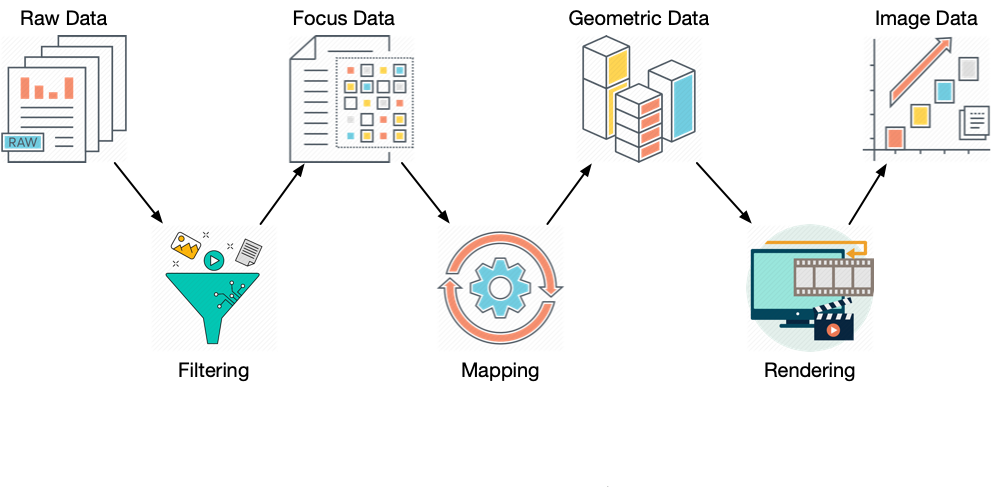
\includegraphics[width=.45\textwidth]{images/pipeline.png}
    \caption{Visualization Pipeline}
    \label{fig:pipeline}
\end{figure}

The filtering step prepares the raw input data for processing through the remaining steps of the pipeline. This is done with respect to the given analysis task and includes not only selection of relevant data but also operations for data enrichment or data reduction, interpolation, data cleansing, grouping, dimension reduction, and others. 

Literally, the mapping step maps the prepared data to appropriate visual variables. This is the most crucial step as it largely influences the expressiveness and effectiveness of the resulting visual representation. 

Finally, the rendering step generates actual images from the previously computed geometry and visual attributes. This general pipeline model is the basis for many visualization systems.

\section{Temporal Display Design}

The bibliography raw data usually is collected in plain text files, and organized by a standard rule, such as BibTex, EndNote etc. In this paper, we use the IEEE VIS conference series data\cite{Isenberg:2016ika} from 1990 to 2016 to illustrate the usage of our method. The data used in our experiments contains IEEE VIS publications, i.e., InfoVis, SciVis, VAST, or Vis. Each record consists of 11 fields, including conference type, publication year, paper title, DOI, abstract, author names, and references (inside this dataset only). In the purpose of exploring research topic, only some fields are involved in the proposed method, which contains the topic features and temporal features. Specifically, the topic features will be extracted from these fields, which are paper title, abstract, and full text if available. The temporal features will be aggregated by the time granularity, which is the 'year' data field in this case. 

\subsection{Data Processing}

The raw data contains topic features and temporal features will be filtered into the focus data by the data processing approach. The raw data is composed by records, which could be distinct from each other by some specific notations or punctuation, such as a semicolon or a line break. Let's define the raw data set is $X := \{X^{(1)},X^{(2)},...,X^{(n)}\}$, where the $n$ is the number of records contained in the raw data, and the $X^{(i)}$ means the $i$th record in $X$ with $1 \leq i \leq n$. 

To show the temporal visualization of the bibliography data set, both the words variable and the times variable should be considered in the data processing approach. To achieve a better visualization presentation with clarity and concision, the method proposed in this paper gives a general pipeline to declare the details of the data processing. 

A ignored word list and a merged word list should be initialized before the data processing approach, and will be continuous updated during the data exploring activity. 

The ignored word list contains frequently used words (such as and, the, because, and so on) or words that you do not want indexed, which will be excluded from the result. The data processing program comes with a default set of ignored words that you can modify as needed. The ignored word list could be defined as $ P := \{P_1,P_2,...,P_m\} $, where $P_i$ with $1 \leq i \leq m$ means a single word will be ignored. 

The merged word list is composed by several word groups, each group contains the words which is a synonym for each other. The merged word list is defined as $ M := \{ M^{(1)}, M^{(2)},...,M^{(n)} \} $, where $M^{(i)}$ with $1 \leq i \leq n$ means the $i$th merged word group. The merged word group is defined as $M^{(i)} := \{ M_1^{(i)},M_2^{(i)},...,M_m^{(i)}\}$. The merged word group is a order-sensitive sequence, all the words in one merged word group will be merged into the first word in the sequence. The merged word list can be initialized by several approaches. One of the most leveraged method is the word distance algorithm, such as the Levenshtein algorithm, which is a string metric for measuring difference between two sequences. Informally, the Levenshtein distance between two words is the minimum number of single-character edits (i.e. insertions, deletions or substitutions) required to change one word into the other. But the word distance algorithm should be applied under supervision. For example, the words "universe" and "university" are quit similar but with very different meaning.





\subsection{Data Mapping}

\subsection{Visualization Result}

\section{Conclusion}



\begin{thebibliography}{1}

\bibitem{dosSantos:2004ck}
S. dos Santos and K. Brodlie, “Gaining understanding of multivariate and multidimensional data through visualization,” Computers \& Graphics, vol. 28, no. 3, pp. 311–325, Jun. 2004.

\bibitem{Isenberg:2016ika}
P. Isenberg, F. Heimerl, S. Koch, T. Isenberg, P. Xu, C. D. Stolper, M. Sedlmair, J. Chen, T. Moller, and J. Stasko, “Vispubdata.org: A Metadata Collection About IEEE Visualization (VIS) Publications,” IEEE Transactions on Visualization and Computer Graphics, vol. 23, no. 9, pp. 2199-2206, Oct. 2016.

\end{thebibliography}
\end{document}


